\documentclass[11pt]{article}
\usepackage{tikz}
\usepackage{mathpazo}

\usetikzlibrary{matrix}

\begin{document}
\thispagestyle{empty}
\begin{center}
\hspace{2cm}\textbf{Fama and Schwet \quad V.S. \quad Baxter and Jermann}
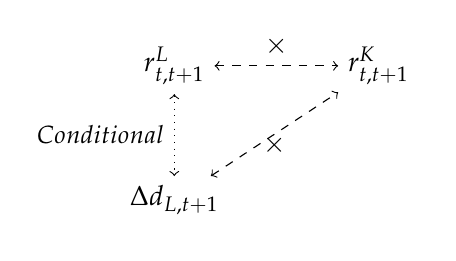
\begin{tikzpicture}
 \matrix (m) [matrix of math nodes,row sep=3em,column sep=4em,minimum width=2em]
  {
     r^{L}_{t,t+1} & r^K_{t,t+1} \\
     \Delta d_{L,t+1} &  \\};

\path[-stealth]
    (m-1-1) edge [dotted,<->] node [left] {\small $ Conditional$}  (m-2-1)
            edge [dashed,<->] node [above] {$\times$} (m-1-2) ;
\path[-stealth]
    (m-2-1) edge [dashed,<->] node [below=-3pt] {$\times$} (m-1-2) ;
\end{tikzpicture}
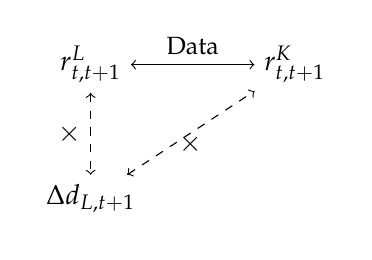
\begin{tikzpicture}
 \matrix (m) [matrix of math nodes,row sep=3em,column sep=4em,minimum width=2em]
  {
     r^{L}_{t,t+1} & r^K_{t,t+1} \\
     \Delta d_{L,t+1} &  \\};

\path[-stealth]
    (m-1-1) edge [dashed,<->] node [left] {$\times$}  (m-2-1)
            edge [<->] node [above] {\small Data} (m-1-2) ;
\path[-stealth]
    (m-2-1) edge [dashed,<->] node [below=-3pt] {$\times$} (m-1-2) ;
\end{tikzpicture}
\end{center}
\end{document}
